\begin{figure}[t]
\centering
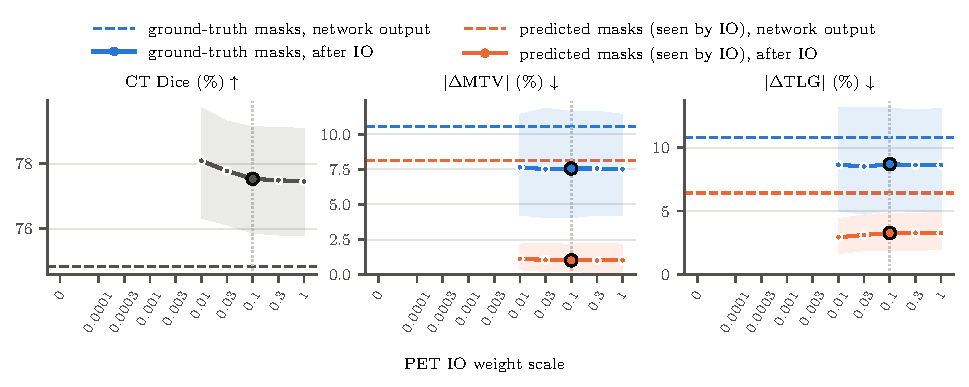
\includegraphics[width=\textwidth]{figures/tradeoff.pdf}
\caption{Effect of the PET-loss weight in instance optimization (IO) on the test set: the network trained without PET losses (T1) is followed by IO with all PET weights scaled by the given factor (0: PET losses off; 1: training-derived weights).
 Metrics are computed on the predicted labels optimized by IO (orange squares; organs: TotalSegmentator, lesions: nnU-Net) and on the provided evaluation labels (blue circles).
 CT Dice includes 28 patients and 38 pairs; metabolic tumor volume (MTV) and total lesion glycolysis (TLG) change include the 26 patients and 30 pairs with lesions in both label sets.
 Solid: after IO; dashed: network output before IO, the same for every factor.
 Outlined point and dotted line: operating point tuned on the validation set.
 Black diamonds: IO with the provided instead of the predicted lesion masks (at $\times0.1$ and $\times1$), evaluated on the provided labels.
 Curves show means over patients after averaging eligible pairs; bands show 95\,\% patient-bootstrap confidence intervals.}
\label{fig:tradeoff}
\end{figure}
